\documentclass[12pt]{article}
\usepackage[utf8]{inputenc}
\usepackage[T1]{fontenc}
\usepackage[a4paper,left=2cm,right=2cm,top=2cm,bottom=2cm]{geometry}
\usepackage[frenchb]{babel}
\usepackage{libertine}
\usepackage[pdftex]{graphicx}
\usepackage{shadow}
\usepackage{amsmath}
\usepackage{amssymb}
\usepackage{graphicx}
\usepackage{textcomp}
\usepackage[colorinlistoftodos]{todonotes}
\usepackage[colorlinks=true, allcolors=black]{hyperref}
\usepackage{tikz}
\usepackage[french,linesnumbered,algoruled]{algorithm2e}
\usepackage{lipsum,xcolor}
\everymath{\displaystyle}


\SetKw{WEntree}{\textcolor{red}{Entrée}}
\SetKw{WEntrees}{\textcolor{red}{Entrées}}
\SetKw{WSaisir}{Saisir}
\SetKw{WInitialisation}{\textcolor{red}{Initialisation}}
\SetKw{WTraitement}{\textcolor{red}{Traitement}}
\SetKw{WSortie}{\textcolor{red}{Sortie}}
\SetKw{WSorties}{\textcolor{red}{Sorties}}
\SetKwIF{Si}{SinonSi}{Sinon}{if}{then}{else if}{else}{endif}
\SetKwFor{Tq}{While}{do}{EndWhile}


\setlength{\parindent}{0cm}
\setlength{\parskip}{1ex plus 0.5ex minus 0.2ex}
\newcommand{\hsp}{\hspace{20pt}}
\newcommand{\HRule}{\rule{\linewidth}{0.5mm}}

\begin{document}

\begin{titlepage}
  \begin{sffamily}
  \begin{center}


    \textsc{\LARGE École nationale supérieure d'électronique, informatique, télécommunications, mathématiques et mécanique de Bordeaux}\\[2cm]

    \textsc{\Large Rapport de projet S6 }\\[1.5cm]

    % Title
    \HRule \\[0.4cm]
    { \huge \bfseries Le jeu Carcassonne\\[0.4cm] }

    \HRule \\[2cm]
      % Author and supervisor
    \begin{minipage}{0.4\textwidth}
      \begin{flushleft} \large
      \textnormal{Réalisateurs :}\\
        Cheikh \textsc{Lilia}\\
          Sandri \textsc{Jordan}\\
            Chlih \textsc{Zakaria}\\
              Naddami \textsc{Anas}\\
        \textit{Promotion 2017-2018}\\
      \end{flushleft}
    \end{minipage}
    \begin{minipage}{0.4\textwidth}
      \begin{flushright} \large
              \emph{Encadrant: } Herbreteau Frédéric \textsc{}
              
      \end{flushright}
    \end{minipage}
    \newline
    \begin{center}
    
\includegraphics[width=0.7\textwidth]{logo.PNG}
     \end{center}

    \vfill

    % Bottom of the page
    {\large 18 mai 2018 }

  \end{center}
  \end{sffamily}
\end{titlepage}
\newpage
\tableofcontents
\newpage

\section{Préambule}

\paragraph{} Dans le cadre du projet du semestre 6 et dans le but d'approfondir nos connaissances en programmation en language C, il nous a été proposé de modéliser un jeu de cartes appelé \textit{Carcassonne}, coder les stratégies necéssaires pour le déroulement du jeu, et définir les structures permettant de représenter le mieux possible les joueurs, le plateau de jeu, les cartes et les coups des joueurs.
L'objectif du projet consiste à implémenter un ensemble de fonctions permettant de faire jouer un nombre quelconque de joueurs à une partie de Carcassonne.

\subsection{Vocabulaire}
\paragraph{} Afin de bien comprendre le fonctionnement du jeu, il est primordial de définir un certain nombre de vocabulaire propre à ce dernier. \\

\begin{itemize}
\item \textit{Deck:} Le deck représente l'ensemble des cartes du jeu qui sont au nombre de 72 cartes. Il existe 24 cartes diffèrentes avec une carte de départ de dos plus foncé nommé CARD\_ROAD\_STRAIGHT\_CITY.\\
\item\textit{Tile:} Il s'agit d'une carte tirée du deck (tuile en français) jouée par l'un des joueurs dans le but de gagner des points.\\
\item\textit{Nodes:}
Les nodes sont les 13 points placés sur chaque carte permettant de faire des connexions entre les diffèrentes cartes pour pouvoir construire des paysages.\\
\item\textit{Meeples:}
Les meeples sont les pions utilisés par les joueurs pour marquer leur territoire.
\end{itemize}

\section{Introduction}

\subsection{Mise en situation}

\paragraph{} Carcassonne est un jeu de société. Le thème est la construction d'un paysage médiéval par la pose de tuiles, incluant des villes fortifiées telles que Carcassonne.
Ainsi, Carcassonne est un jeu où l'on construit le plateau de jeu au cours de la partie. Des points sont attribués en fonction de la taille des combinaisons créées — villes, champs, routes, abbayes.\\

Le jeu commence avec une seule tuile, les autres étant dans une pioche. Chaque joueur à tour de rôle pioche une tuile et doit la placer en respectant les tuiles déjà en place : les villes et les routes ne peuvent être coupées.\\

Après avoir placé sa tuile, et uniquement à ce moment-là, le joueur peut s'il le souhaite placer un pion, désigné par le terme \textit{meeple} en anglais, sur une des parties de cette tuile (morceaux de villes ou de champs, tronçons de chemins, abbayes). La ville, le champ, l'abbaye ou le chemin formé par les éléments contigus deviennent alors la propriété exclusive de ce joueur, et personne, pas même le propriétaire, ne pourra y placer d'autre pion en l'agrandissant par une nouvelle tuile contiguë. Cependant, une nouvelle tuile peut réunir des parties disjointes sur lesquelles il y a déjà des pions. C'est alors le joueur qui a le plus de pions sur le domaine en question qui devient le propriétaire de l'ensemble (si les joueurs sont à égalité, le terrain appartient autant à chacun).\\

Quand une route, une ville ou une abbaye est complétée, son ou ses propriétaires comptent leurs points (chaque tuile a une certaine valeur), et récupèrent leurs pions. Les pions placés sur les champs y restent jusqu'à la fin du jeu.\newline

Le jeu est terminé quand toutes les tuiles ont été placées. On compte alors des points pour les abbayes, les champs, les routes et les villes non complétées.\newline

\subsection{Les règles du jeu}

\paragraph{} Le jeu \textit{Carcassonne} est géré par un ensemble de règles qu'on pourrait résumer de la manière suivante:

\begin{itemize}

\item Au début du jeu, on dispose d'une pile de 72 cartes bien mélangées entre elles (24 types de cartes, chaque type apparaîssant un nombre bien determiné de fois dans la pile). Ces cartes présentent des paysages (chemins, villes, pré, abbaye). La première carte a être posé sur le plateau est CARD\_ROAD\_STRAIGHT\_CITY, le plateau se construit alors autour de cette carte.

\item Chaque joueur pioche une carte à tour de rôle, la pose sur le plateau de jeu de telle manière qu'elle soit accolée à au moins une autre carte figurant sur le plateau et qu'elle forme avec cette carte là une tranche d'un paysage. Étant donné les règles du jeu, il est presque impossible que le joueur ne puisse pas placer une carte. Mais si le cas se présente il doit mettre cette carte paysage de côté et piocher une nouvelle carte.\\

\begin{figure}
	\begin{center}
	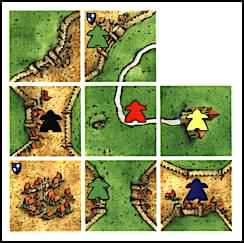
\includegraphics[width=0.3\textwidth]{completer.jpg}
	\end{center}
    \caption{Les différents paysages (villes,chemin,abbaye)} \label{figure1}
\end{figure}

\item Une fois qu'il a pioché une carte , le joueur peut positionner un unique \textit{partisan} sur une portion de la carte qu'il vient de déposer sur le plateau. Chaque joueur dispose de 8 \textit{pions} de même couleur. L'emplacement choisi par le joueur pour son \textit{partisan} défini la nature de celui-ci . Par exemple, un \textit{chevalier} devrait être placé dans le quartier d'une ville , un \textit{voleur} sur un chemin, un paysan dans un pré et un \textit{moine} dans une abbaye. Cependant, il existe certaines contraintes qui doivent être prises en compte lors du choix de l'emplacement d'un \textit{pion}. 				
En effet, le joueur ne peut placer son partisan sur la partie de son choix que si il n'y a pas encore d'autres partisans dans les villes, sur les chemins ou dans les prés qu'il a complétés avec sa carte de paysage et ceci indépendamment de la distance qui le sépare de l'autre partisan. Par exemple, s'il decide de placer un chevalier, il doit s'assurer que dans ce paysage là, il n'existe aucun chevalier. Dans le cas contraire, il doit choisir un nouvel emplacement pour son \textit{pion}.\newline

\begin{figure}
\begin{center}
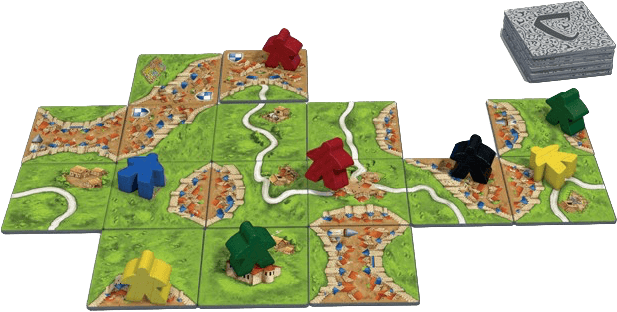
\includegraphics[width=0.5\textwidth]{meepleonmap.png}
\end{center}
\caption{Modélisations des pions sous formes de bonhommes colorés} \label{figure2}
\end{figure}

\item Une fois qu'un paysage est complet sur le plateau de jeu, il faut évaluer les points qui en découlent et les affecter au total de points du/des joueurs en question. Les points attribués dependent de la nature du paysage construit, du type de pions placés ainsi que du nombre de cartes des joueurs participant à la création de ce paysage.\newline
Le calcul des points se fait suivant les règles suivantes:\newline
\underline{RÈGLE 1 :} Une ville est dite achevée si le paysage formé est un espace fermé et si les extrémités de ce paysage sont des remparts. Des points seront attribuées au joueur dont le chevalier figure sur le paysage. Il reçoit 2 points par carte utilisée pour former la ville aussi bien que 2 points par symbole. Une exception s'applique dans le cas où la ville est formée par deux cartes seulement, en effet, le joueur en question ne reçoit que 2 points.\newline

\begin{figure}[!h]
\begin{center}
\begin{tabular}{cc}
   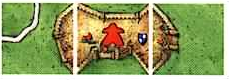
\includegraphics[width=0.42\textwidth]{ville-8-pt.png} &
   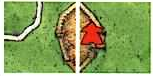
\includegraphics[width=0.3\textwidth]{ville-2-pt.png} \\
\end{tabular}
\end{center}
\caption{Construction de villes par deux ou plusieurs cartes } \label{figure3}
\end{figure}

\textsf{Ici le joueur en question reçoit 8 points dans le cas de la figure \ref{figure3} (gauche) alors qu'il n'en reçoit que deux dans le deuxieme (droite).}\newline
Il peut toute fois arriver qu'il y ait plusieurs joueurs dans la même ville dans ce cas le joueur qui possède le plus de chevalier dans cette ville remporte les points. En cas d'égalité les joueurs concernés reçoivent la totalité des points.
Dans le cas où il y a plusieurs chevaliers sur une même ville , c'est le joueur ayant le plus grand nombre de chevaliers qui emporte la totalité des points. En cas d'égalité, chacun des joueurs concernés reçoit la somme des points. \newline

\underline{RÈGLE 2 :} Un chemin est considéré comme achevé lorsqu'il est continu et cloturé sur ses 2 extrémités par une ville, un carrefour ou une abbaye. Le joueur, dont le voleur se trouve sur le chemin, compte alors les cartes qui lui ont permis de le créer et il reçoit le nombre de points correspondant.\newline

\begin{figure}[!h]
\begin{center}
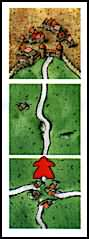
\includegraphics[width=0.15\textwidth]{route_achevee.jpg}
\end{center}
\caption{Route achevée} \label{4}
\end{figure}

Ici, le joueur remporte 3 points dans le cas de la Figure \ref{4} la route est fermée est cloturé par un carrefour. Dans le cas où il y a plusieurs voleurs sur un même chemin, c'est le joueur ayant le plus grand nombre de voleurs qui emporte la totalité des points. En cas d'égalité, chacun des joueurs concernés reçoit la somme des points.\\

\newpage \underline{RÈGLE 3 :} Le pré est formé de plusieurs cartes de paysage mises les unes à cotés des autres pour obtenir un dessin continu. Pendant la partie, on ne peut pas donner une valeur aux prés ou aux partie de prés, mais on peut y placer des paysans. On ne reçoit les points correspondant qu'à la fin de la partie. Les paysans restent par conséquent, sur les cartes de paysage pendant toute la partie et les joueurs ne peuvent pas les récupérer. Les prés sont délimités par des chemins, des villes et le bout des cartes sur la table. \newline

\begin{figure}[h!]
\begin{center}
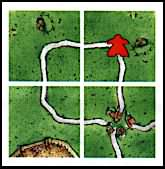
\includegraphics[width=0.3\textwidth]{pre_achevee.jpg}
\end{center}
\caption{Pré achevée} \label{5}
\end{figure}

Dans le cas de la Figure \ref{5} le joueur ne remportera pas de point puisque que pour marquer des points avec un pion paysan il faut que le champ de ce pion touche une ville fermée dans ce cas c'est 4 points par ville finie. Le champ est fini mais le joueur récupère pas son pion La même règle s'applique en cas d'égalité celui qui a le plus de paysan dans le champ remporte les points, si même nombre de pions les 2 joueurs remportent la totalité des points\\

\underline{RÈGLE 4 :} Une abbaye est dite achévée si le paysage obtenu présente un batiment entouré par huit cartes. Dans ce cas là c'est le joueur dont le moine est placé dans l'abbaye qui reçoit un point pour chaque carte entourant l'abbaye et un point pour le pion, donc au total 9 points.\newline

\underline{RÈGLE 5 :} Si un joueur a terminé une ville, un chemin ou une abbaye en plaçant sa carte, il doit tout de suite compter les points correspondants. \newline

\underline{RÈGLE 6 :} Vu que chaque joueur dispose d'un nombre réduit de \textit{pions}, le jeu permet, à chaque fois qu'il y a une évaluation d'une ville, d'un chemin ou d'une abbaye, de récupérer les partisans placés, sur les cartes de paysages correspondantes. Au tour suivant, les joueurs peuvent les réutiliser sur de nouvelles cartes de paysage qu'ils décident de placer.\\

\item Après la pioche de la dernière carte du jeu et le placement d'un pion ainsi que la mise à jour des points des joueurs si necessaire vient la dernière étape du jeu, qui est l'évaluation finale. Il s'agit ici d'attribuer des points aux joueurs, selon l'emplacement de leurs pions, pour les villes, abbayes et chemins incomplets. 

\end{itemize}
\begin{figure}[h!]
\begin{center}
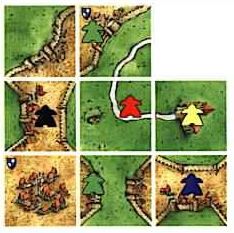
\includegraphics[width=0.24\textwidth]{eval-final.png}
\end{center} 
\caption{Paysage incomplet} \label{figure5}
\end{figure}

\paragraph{} Dans la figure \ref{figure5} ci-dessus, le joueur qui a déposé le voleur aura 3 points pour le chemin inachevé alors que le joueur ayant déposé le moine dans l'abbaye aura 5 points pour l'abbaye inachevée.

\subsection{Objectif du projet}

\paragraph{} L’objectif  de  ce  projet  est  d'écrire  un  code  en  C  fidèle  aux  règles  du  jeu Carcassonne. D’autres objectifs sont de produire un code propre, mais également des fonctions avec une complexité, nous permettant de faire tourner le jeu en un temps d’exécution correct. Pour cela notre projet tournera autour de la question : Comment rendre le code optimisé et fidèle aux règles du jeu ?

\section{Implémention} 

\subsection{Intéraction client/serveur}

Le jeu Carcassonne comporte beaucoup de règles que les joueurs se doivent de respecter pour cela nous mettrons en place un serveur qui jouera le rôle d'arbitre pour chaque coup joué et mettra à jour le plateau. Chaque joueur disposera de son propre plateau qui sera mis à jour en récupérant les coups valides des autres joueurs lorsque le joueur en question jouera. Seul le serveur dispose d'un plateau qui évolue à la fin de chaque coup joué par un joueur, et seul ce plateau compte pour l'arbitrage. Cependant si les joueurs jouent des coups valides ils auront le même plateau.\\

Un joueur qui ne respecte pas les règles sera lourdement sanctionné, le serveur l'éjectera du jeu sans sommation, et ne comptabilisera pas son coup sur le plateau, mais on l'ajoutera aux coups joués en tant que coup invalide pour garder sa trace. Même si le joueur éjecté est gagnant vu son grand nombre de points, c'est le deuxième joueur qui possède le plus de point qui sera nommé vainqueur de la partie. On pourrait permettre au joueur de re-jouer mais le joueur pourrait s'amuser à ne pas faire avancer la partie en faisant que des mauvais coups. De plus cela facilite les modifications des plateaux de jeux des joueurs.

\subsection{La boucle globale du jeu}

\paragraph{} Pour aborder le jeu et modéliser les intéractions entre les joueurs et le serveur, on a opté pour un algorithme général qui suit la démarche du pseudocode suivant :

\LinesNumbered
\DontPrintSemicolon
\begin{algorithm}
\For{each player}{
	{$player \leftarrow initialise();$};
}
{$deck \leftarrow fill\_deck();$}\\
\For{each player}{
	\Tq{(!\ is\_empty(deck))\ and\ (remaining\_players(players) > 1)}{
    	{$card \leftarrow draw\_card();$}\\
    	\Si{playable(card)}{
    		\Si {(!\ valid\_move(move\_player))}{
   				 {$eject\_player(player);$}
    			}
    		{enqueue(move\_player, moves);}\\
   		    {$player \leftarrow compute\_next\_player();$}\\
    	}
	}	
}
\For{each player}{
	{$player \leftarrow finalise();$}
}
\caption{\textit{Main loop of the game}} \label{1}
\end{algorithm}

\paragraph{}Les différentes fonctions figurant dans la boucle principale nous orientent vers la considération de différents types abstraits de données (TAD) pour modéliser chaque partie du jeu. Ces TAD seront exposés dans la section suivante.

\section{Définitions des types abstraits de données nécessaires pour la modélisation du jeu}

À l'aide de la boucle de jeu, on va déterminer petit à petit les fonctions dont on a besoin d'implémenter pour coder le jeu et également les TAD qu'ils leurs sont associés.

\newsavebox{\fmbox}
\newenvironment{fmpage}[1]
     {\begin{lrbox}{\fmbox}\begin{minipage}{#1}}
     {\end{minipage}\end{lrbox}\shabox{\usebox{\fmbox}}}
     
\subsection{Les fonctions du TAD deck} 
Au cours du jeu, les joueurs doivent tirer à tour de rôle une carte parmi un deck de 72 cartes, c'est la première instruction dans la boucle While. On a besoin de fonction permettant d'intéragir avec le deck. Pour cela nous mettrons en place les fonctions de base suivante :

\begin{itemize}
\item \textit{struct deck *init\_deck()}: fonction qui crée un deck vide, le remplit  avec les cartes du jeu et le mélange.\\
\item \textit{enum card\_id  draw\_card(struct deck *deck)} : fonction qui renvoie la carte sur le dessus du deck (la nouvelle carte à piocher).\\
\item \textit{int deck\_is\_empty(struct deck *deck)}: fonction qui renvoie TRUE si le deck est vide, FALSE sinon.\\
\item \textit{void deck\_free(struct deck *deck)} : fonction qui libère la mémoire alloué par le deck.\\

\end{itemize}

\subsection{Déduction d'une structure deck}

\paragraph{} On a besoin d'un tableau d'énumération pour stocker les cartes du jeu, ainsi que d'un repère pour savoir quelle carte est la suivante, on implémentera la structure suivante :\\ 

La structure deck se composera d'un tableau d'énumération \textit{card\_id} contenant les 72 cartes du jeu \textit{next\_card} indiquant la position de la carte suivante à tirer.

On a opté pour une structure semblable à la structure d'une pile. En effet, le champ contenant le tableau des cartes est notre pile qui va contenir toutes les cartes, et le champ next\_card est un entier qui va mémoriser le sommet de la pile, indiquant l'emplacement de la première carte à piocher à chaque tour de jeu. Au début du jeu, cet entier est initialisé à 0, puis incrémenté à chaque fois qu'on pioche une carte. \\

\subsection{Les fonctions du TAD moves}

On a besoin de mémoriser les coups joués par les joueurs pour pouvoir valider les coups suivants mais également pour pouvoir compter les points par la suite. Une autre fonctionnalité de ce TAD est de transmettre l'information entre le serveur et le client. Pour cela nous aurons besoin des fonctions suivantes :

\begin{itemize}
\item \textit{struct moves *init\_moves():} fonction qui crée une structure moves et initialise les champs de la structure.\\
\item \textit{struct move *last\_n\_moves(struct moves *moves, int number\_of\_moves):} fonction qui renvoie les coups du dernier tour joué.\\
\item \textit{int add\_move(struct moves *moves, struct move *move):} fonction qui ajoute un coup joué à la liste des coups précédents.\\
\item \textit{void free\_moves(struct moves *moves:} fonction qui libère l'espace allouée à la structure moves.\\
\end{itemize}

\subsection{Déduction d'une structure moves}

\paragraph{}
Lorsqu'un coup est joué il faut retenir plusieurs informations. Quelle est la carte posée ? Sa position sur le plateau, l'emplacement d'un possible pion, etc. De plus cette structure nous sert de passerelle entre le client et le serveur on y rajoute alors un champs pour vérifier la validité du coup. Il y aura donc 2 structures pour les coups joués. La structure \textit{move} qui va contenir les informations importantes à retenir lorsqu'un coup est joué et la structure \textit{moves} qui est un tableau de structure move pour mémoriser les coups. On définira les structures suivantes: \\

La structure moves comportera un tableau contenant les struct move des joueurs, ainsi qu'un champ \textit{count\_move} qui enregistre le nombre de struct move comprisent dans le tableau.

Ainsi que la structure \textit{move} suivante :

La structure move contient un booléen qui indique TRUE si le coup est validé par le serveur FALSE sinon. Un champ \textit{id\_player} qui renseigne l'id d'un joueur. Une énumération \textit{card\_id} qui est l'id de la carte jouée. Une struct position qui est la position de la carte sur le plateau. Une enum direction qui indique le nord de la carte et une enum place qui donne la position du pion posé sur la carte et \textit{NO\_MEEPLE} s'il n'y en a pas.

\subsection{Les fonctions du TAD players}

\paragraph{} Pour le déroulement du jeu, on a besoin de charger les bibliothèques des joueurs, vérifier s'ils sont en vie, éjectés du jeu ou non et calculer les points accumulés lors de chaque tour. Les principales fonctions dont on a besoin sont les suivantes : \\

\begin{itemize}
\item \textit{struct players *init\_players()}: fonction qui alloue de la mémoire pour la structure \textit{player} et initialise les differents champs de la structure.\\
\item \textit{unsigned int compute\_next\_player(struct players *players, struct player *player)}: fonction qui renvoie l'identité du prochain joueur en vie qui va jouer.\\
\item\textit{void eject\_player(struct players *players, struct player *p)} fonction qui exclut un joueur du jeu une fois qu'il a joué un coup invalide.\\
\item\textit{int remaining\_players(struct players *players)} fonction qui retourne le nombre de joueur encore en vie, les joueurs exclus comptent pour morts.\\
\item \textit{void free\_players(struct players *p)} : fonction qui libère la mémoire allouée aux joueurs.\\
\end{itemize}

\subsection{Déduction d'une structure players}

Pour faciliter la communication entre le serveur et le client, il est pratique d'avoir des pointeurs de fonctions pour cela on met en place la structure suivante : \\

La structure \textit{player\_base} contient un pointeur de fonction vers la fonction \textit{initialise} du client, ainsi qu'un pointeur de fonction vers la fonction play du joueur, qui lui permet de renvoyer son coup, un pointeur de fonction qui renvoie le nom du joueur, un pointeur de fonction vers la fonction \textit{finalise} du client et handle un pointeur qui récupère ce que retourne la fonction \textit{dlopen} qui charge les bibliothèques.

\paragraph{}Cette structure nous sera trés utile vu qu'elle stocke les adresses des fonctions à charger pour un client.
Ainsi, pour charger la bibliothèque relative à un client, on a codé une fonction auxilière \textit{load\_functions(void *player, struct player\_base *base)} qui accède à la bibliothèque d'un joueur et initialise les champs de la structure \textit{player\_base}. Cette fonction nous sera utile pour le codage de \textit{init\_players()}.\newline

Certaines informations relatives aux joueurs en plus de la structure player\_base doivent être mémorisées, pour cela on met en place une structure \textit{player} comme suit :\\

La structure player contient un pointeur vers la structure player base du joueur. Un booléen qui indique si le joueur est en vie l'id du joueur. Le nombre de pions qui restent au joueur, et le nombre de points qu'il génère au cours de la partie.

\paragraph{} Le premier champs de la structure est un pointeur vers \textit{struct player\_base} . Ceci nous permet de stocker toutes les adresses des fonctions des clients participant aux jeu.

Afin de repérer les joueurs encore en vie, on a ajouté le champ \textit{int player\_alive} à la structure \textit{player}: le joueur correspondant est vivant si ce champ vaut TRUE et exclu du jeu (suite à un coup invalide) ou mort si la valeur du champ est FALSE . Les champs \textit{number\_of\_meeples} et \textit{points} nous servirons pour le comptage des scores et la détermination du joueur gagnant. 

\paragraph{} À partir de cette structure et de la même manière que pour la structure move il sera plus aisé de stocker les joueurs dans un tableau de joueurs.\\

La structure players contient un tableau de structure player et un entier \textit{number\_of\_players} qui indique le nombre de joueurs initials en début de partie.

\section{Définition des types abstraits de données permettant de valider les coups joués}

\subsection{Les fonctions du TAD tile}

Jusqu'à présent, l'ensemble des structures réalisées permettent de partager des informations sur un coup joué entre le serveur et le client mais aucune vérification n'est effectuée. Les joueurs peuvent placer des cartes sur le plateau comme bon leur semble et il en est de même pour les pions. Il est alors nécessaire de rajouter des fonctions qui vont nous permettre de vérifier les coups joués. Pour cela nous aurons besoin de définir les fonctions qui intéragissent avec les tuiles, nous définirons les fonctions suivantes : 

\begin{itemize}
\item \textit{struct tile* init\_tile() :} fonction qui alloue de la mémoire et initialise une tuile\\
\item \textit{void free\_tile(struct tile *tile):} fonction qui libère la mémoire allouée à une tuile.\\
\item \textit{
boolean is\_empty\_tile(struct tile *tile)}: fonction qui retourne TRUE si la tuile n'est pas encore initialisé.\\
\item \textit{match\_side(struct tile* tile1, struct tile *tile 2):} fonction qui vérifie si 2 cartes adjacentes peuvent être connectées (vérification d'une seule face)
\end{itemize}

\subsection{Déduction d'une structure tile}

\paragraph{} Quelles sont les informations qu'une tuile doit retenir ? Sa position, le type de décor que possède chaque côté de la carte. Nous définissons une énumération permettant de donner un nom au type de décor différent.\\

L'énumération landscape contiendra ROAD, PLAIN, CITY, CROSSROAD et ABBEY.\\
Puis la structure tile contiendra un tableau d'énumération landscape des 13 points primordiaux de la carte voir figure \ref{a}, une structure position avec les coordonées x et y de la carte sur le plateau de jeu, l'orientation du nord de la carte, et son nom.

\begin{figure}[!h]
\begin{center}
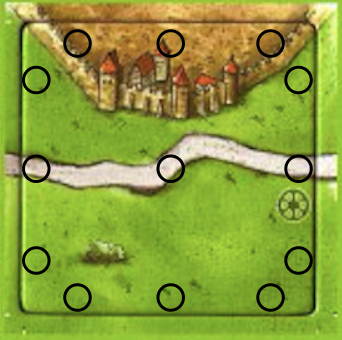
\includegraphics[width=0.3\textwidth]{carte1.png}
\end{center}
\caption{Représentation des 13 points représentant une carte} \label{a}
\end{figure}

L'orientation de la carte et son nom nous servent particulièrement pour l'affichage.

\subsection{Les fonctions du TAD set\_graph}

Une fois que nous avons défini ces tuiles nous allons les stocker dans un tableau. Cela va nous permettre d'avoir accès à ces tuiles pendant la partie et de vérifier que les coups joués par les joueurs sont valides. Nous aurons besoin de ces fonctions :

\begin{itemize}
\item \textit{struct graph *init\_graph():} fonction qui crée un nouveau graphe et l'initialise.\\
\item \textit{int add\_tail\_tile(struct graph *graph, struct move *move):} fonction qui ajoute à la fin du tableau une tuile.\\
\item \textit{int *is\_playable(struct graph *graph, enum card\_id card):} fonction qui vérifie si la carte tirée dans la pioche est jouable à ce stade du jeu\\
\item \textit{struct graph *valid\_move\_card(struct graph *graph, struct move *move):} fonction qui vérifie si la carte placée par le joueur est valide.\\
\item \textit{struct graph *free\_graph():} fonction qui libère le graphe.\\

\end{itemize}

\subsection{Déduction d'une structure set\_graph}

\paragraph{} la structure set\_graph en découle d'elle même, elle se rapproche de la structure \textit{moves} présentée plutôt.

Cette structure contiendra les champs suivants : Un tableau qui contient les tuiles du jeu au fur et à mesure qu'elles sont jouées et le nombre de tuiles présentent dans ce tableau.

\subsection{Les fonctions du TAD node}

Pour vérifier la validité du placement des pions par le joueur, la structure tile n'est plus suffisante. Il ne suffit plus de savoir si les côtés des cartes concordent mais si une zone est libre ou occupée par un pion adverse. 

\begin{itemize}
\item \textit{struct node *init\_node():} qui retourne une structure node alloué et initialisée.\\
\item \textit{int node\_connection(struct node *node1, struct node *node2):} qui lie 2 nodes entre elles.\\
\item \textit{int node\_disconnection(struct node *node1, struct node *node2):} qui délie 2 nodes entre elles.\\
\item \textit{int is\_meeple\_in\_area(struct node *node):} qui parcours le graphe dont la node fournie en fait partie et renvoie si sur le chemin il y avait un pion ou non.

\end{itemize}

\subsection{Déduction d'une structure node}

La structure node a besoin de tous les renseignements que doit savoir une node de la carte pour pouvoir parcourir un graphe c'est à dire qu'elles sont les nodes suivantes liées à cette node, quelle est leur landscape, s'il y a un pion et a qui appartient t-il ?\\

La structure node se compose comme suit : un enum landscape qui indique la catégorie de la node, un booléan qui indique si la node contient un pion et un champ \textit{id\_player} qui indique à qui appartient le pion si le booléen précedent est vrai, un tableau de pointeur vers des struct node voisines pour permettre le parcours de graphe et un entier indiquant le nombres de nodes voisines, pour faciliter le parcours de graphe.

\section{Liaisons entre les TAD}

Les TAD se divisent en 2 catégories les TAD qui intéragissent entre le client et le serveur et permettent également d'entretenir le plateau, et les TAD qui permettent seulement d'entretenir le plateau. La première catégorie des TAD sont des TAD qui ne sont pas imbriqués les uns dans les autres, tandis que dans la deuxième catégorie on a une inclusion des TAD par ordre d'abstraction.
Tout d'abord nous avons vu que dans la structure set\_graph on avait un tableau qui contenait les tuiles du jeu au fur et à mesure qu'elles sont posées, et ces tuiles comportes 13 nodes sur les points essentiels de la carte. On a alors une inclusion de la structure node dans la structure tile et de la structure tile dans la structure set\_graph.

\section{Modifier les structures : les fonctions importantes}

Certaines fonctions permettent d'intéragir entre le client et le serveur et d'autres fonctions permettent de vérifier les coups joués par le client. Un vrai réseau se crée entre les tuiles au fur et à mesure de l'avancée de la partie. Par exemple pour vérifier qu'un coup est valide, on appelle la fonction \textit{valid\_move} qui se décompose en 2 appels. Un appel à la fonction \textit{valid\_move\_card} et un appel à la fonction \textit{valid\_move\_meeple}.\\

La fonction \textit{valid\_move\_card} permet de vérifier qu'une carte est posée au bonne endroit. Tout d'abord à l'aide la fonction \textit{match\_card} on vérifie que les cartes adjacentes à la nouvelle carte posée sont du même landscape si c'est le cas les connexions entre les cartes sont réalisées comme sur la figure \ref{b}:

\begin{figure}[!h]
\begin{center}
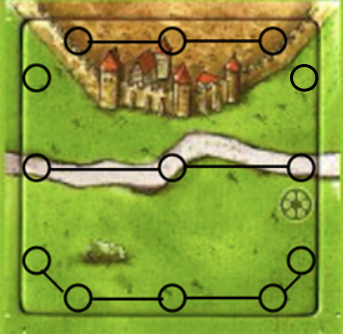
\includegraphics[width=0.3\textwidth]{carte2.png}
\end{center}
\caption{Représentation des liaisons entre les 13 points représentant une carte} \label{b}
\end{figure}

C'est la fonction \textit{add\_tail\_tile} qui s'occope d'ajouter la carte dans le tableau des cartes, elle appelle ensuite \textit{add\_card\_connexion} qui fait la connexion entre les cartes et plus précisement les nodes. La fonction \textit{valid\_move\_card} est en $\Theta$(nombre de voisin) c'est à dire en $\Theta$(1). L'ajout d'une nouvelle carte dans le tableau est également en $\Theta$(1) du fait que l'on tient à jour le nombre de tuiles présentent dans le tableau. Les connexions entre les cartes sont également en $\Theta$(1) puisqu'on relie les nodes voisines par des pointeurs et ses nodes sont mémorisées dans un tableau dans la structure node.\\

La fonction \textit{valid\_move\_meeple} permet de vérifier qu'un pion poser sur une carte à le droit d'être poser en fonction des autres pions sur le plateau, mais aussi en fonction du tableau \textit{allowed\_positions} qui donne les positions permissent d'un pion sur chaque carte. Enfin, elle vérifie si le joueur à assez de pion pour jouer et met à jour le nombre de pions du joueur en sa possésion. La vérification de la validité de ce pion dépend des autres pions sur le plateau. À l'aide des liaisons faites entre les cartes, on peut parcourir un graphe en fonction d'une node données et vérifier dans chaque node s'il elle contient un meeple si c'est le cas le coup n'était pas valide.\\
Le parcours du graphe est un parcours en profondeur, comme le montre l'algorithme \ref{z}.
À l'aide d'une pile on empile les voisins de la node de départ puis on dépile la dernière node ajoutée et on réalise le traitement souhaité, ici regarder s'il y a un pion posé sur cette node. On continue l'algorithme jusqu'à ce que la pile se vide. La compléxité est en $\Theta$(|V|) où |V| représente le nombre de nodes.

\LinesNumbered
\DontPrintSemicolon
\begin{algorithm}

{$stack \leftarrow init\_pile();$}\\
{$visited \leftarrow init\_pile();$}\\
{$add\_pile(stack, n\_check);$}\\
{$add\_pile(visite, n\_check);$}\\
\Tq{(!\ is\_empty(pile))}{
	{$n\_check \leftarrow dequeue\_pile();$}\\	
    	\Si{is\_meeple(n\_check)}{
			{$free\_pile(stack);$}\\
            {$free\_pile(visited);$}\\
            {$return\ TRUE;$}\\
    		}
    		\For{each neighbour nodes}{
            \Si{!\ (find\_pile(visited, neighbour(n\_check)))}{
   		    	{$add\_pile(stack, neighbour(n\_check));$}\\
                {$add\_pile(stack, neighbour(n\_check));$}\\
    	}
        }
{$free\_pile(stack);$}\\
{$free\_pile(visited);$}\\
{$return\ FALSE;$}\\
}	
\For{each player}{
	{$player \leftarrow finalise();$}
}
\caption{\textit{is\_meeple\_in\_area(struct node *n)}} \label{z}
\end{algorithm}

\newpage

\section{Implémenter une stratégie de jeu pour les joueurs}

Carcassonne est un jeu de pose de tuiles où l'objectif est de marquer le plus de points. Chaque joueur est répresenté par une bilbiothèque différente et peut donc avoir sa propre stratégie.\\

\subsection{Les stratégies implémentées par nos joueurs}

La stratégie implémentée dans notre version est un joueur qui jouerait d'une manière bien particulière, plus précisement un joueur qui poserait sa carte dès qu'il trouve une position valide. Pour cela, on appelle la fonction \textit{search\_valid\_position\_card}, qui réalise un parcours du tableau contenant les tuiles posées sur le plateau et vérifie à l'aide de \textit{is\_connectable} si une carte peut se placer à côté d'autres cartes peu importe son orientation.\\

\LinesNumbered
\DontPrintSemicolon
\begin{algorithm}
{$tile \leftarrow init\_tile(card, direction, position);$}\\
\For{all tiles in graph}{\For{all neighbours of this tile}{
{$tile \leftarrow neighbour\_pos(tile)$;} \\
\Si {is\_empty\_tile(neighbour(tile))\ and\ is\_connectable(graph, tile)}{
{$update\_pos(move);$}\\
{$free(tile);$}\\
{$return move;$}}
}
}{{$free(move);;$}\\
{$return move;$}}\;
\caption{\textit{struct move search\_valid\_position\_card\ (struct\ graph *g,\ struct\ move *m)}} \label{2}
\end{algorithm}

Cet algorithme est en $\Theta({nombre\_de\_tuiles^2} * nombre\_de\_voisins)$. La recherche du voisin pour mettre à jour tile pourrait se faire en temps constant si chaque carte posée sur le plateau pointait vers son voisin direct. Il suffirait d'ajouter la carte au graphe et de faire les liaisons $\Theta(1)$ puis d'acceder aux voisins $\Theta(1)$. L'algorithme serait alors en $\Theta$(nombre\_de\_tuiles * nombre\_de\_voisins).

La méthode utilisée pour la pose des pions est semblable sauf que cette fois ci on parcours le tableau \textit{allowed\_positions} qui nous donne les positions valides pour la pose d'un pion sur chaque carte et lorsqu'il repère une position correcte, il pose le pion.

\subsection{Les stratégies implémentables pour une version améliorée}

\begin{itemize}

\item Méthode 1 : Il serait possible alors d'implémenter une strategie réellement aléatoire. On pourrait par exemple mémoriser dans un tableau toutes les positions valides et choisir l'une de ces positions aléatoirement pour poser la carte et pareillement pour le pion.\\

\item Méthode 2 : Une autre méthode serait quand un joueur qui fait un peu plus attention aux points, c'est à dire qu'il cherche à marquer des points, préfererait une position plutôt qu'une autre. Par exemple toujours en récupérant le tableau des positions valides pour une carte, on peut vérifier pour chaque carte si elle achève une route ou une ville ou poser un pion sur une ville ou une route qui ne comporte pas encore de pions, en utilisant le parcours de graphe décrit précédement. Pour la pose des pions, le joueur pourrait préférablement poser son pion sur une abbaye ou une ville lorsqu'il joue une nouvelle carte.\\

\item Méthode 3 : Une dernière méthode serait un joueur qui essaye de bloquer les coups des autres joueurs par exemple il pourrait agrandir une ville ou une route où un joueur adverse se trouve. Il pourrait également chercher à ne pas poser de carte à coté d'une abbaye adversaire. S'il ne peut pas bloquer un autre joueur adopterait la méthode 1 ou 2.\\

\end{itemize}

\section{Compter les points des joueurs}

\paragraph{} Compter les points des joueurs sur Carcassonne est compliqué, il faut parfois les ajouter en cours de partie et parfois en fin de partie.\\

Pour compter les points des routes il s'agirait de faire un parcours des nodes dans les tuiles en rajoutant un champ indiquant si la node représente une route qui se termine, et de vérifier que dans le graph des routes il y ait bien 2 routes qui se terminent.\\

Pour compter les points dans une ville la méthode est encore une fois similaire un parcours de graphe à partir d'une node ville. Cependant, il faudra vérifier en plus que la ville n'est pas un trou en son centre et que les bords de la carte soient bien des remparts.

Pour compter les champs, on réalise encore une fois un parcours, mais cette fois-ci il faudrait avoir connaissance des villes qui sont en contact avec le champ, en rajoutant un champ dans la structure node.

Pour compter les abbayes on pourrait rajouter un champ dans la tuile d'une abbaye comptant le nombre de cartes voisines de celle-ci.

\section{Conclusion}

\subsection{Résultats expérimentaux}

\paragraph{} À ce stade du code, le jeu est prêt à lancer une partie de Carcassonne sans la pose des pions. De nombreuses parties ont été lancées afin de vérifier que le déroulement de chaque partie est cohérent avec les règles énoncées plutôt. Une version avec les pions est disponible sur le dépôt sous le nom de \textit{carcassonne\_meeple} mais n'est pas totalement fonctionnelle. La pose des pions reste encore fausse à certains moments.

\subsection{Le code fourni atteint-il l'objectif fixé ?}

L'objectif fixé était de fournir un code optimisé et fidèle aux règles du jeu. Les règles sont respectées dans un sens où effectivement l'algorithme ne prend pas en compte les pions, mais le code fourni ne contredit pas les règles établies pour la pose des cartes. Le code proposé a été réalisé dans un souci de clarté et de propreté. Autant de fonctions auxiliaires que possible ont été réalisées, afin de rendre chaque fonction claire, précise, et facile à comprendre. Les noms des variables et des fonctions ont été choisies avec soin, toujours dans le but de proposer le code le plus clair et compréhensible possible. Des commentaires ont été écrits aux endroits clés du code pour des raisons de clareté et de compréhension. De plus, de nombreuses séparations du code en différents fichiers (e.g. *.c, *.h) ont été réalisées, afin de rendre la manipulation du code plus claire, et sa maintenance plus facile.
  Le codage systématique des fonctions de test permet aussi d'affirmer que le code produit répond aux exigences, ainsi qu'aux règles du jeu, de manière fidèle. Ainsi, même si des optimisations au niveau algorithmique sont envisageables, le code proposé semble en un sens répondre à l'objetif fixé. 





\end{document}

le pb
comment on a resolu nos pb
dessiner sur le tableau / ecrire au tableau


Plan : 
	preambule
	vocabulaire
    
    tile
	nodes/set_dynamic
    set_graph(rajoutons une couche d'abstraction en plus)
    
    comment sont reliées les structures ?
    developper les fonctions importantes des TAD (en particulier le 
    parcours de graph)
    
    Methodes alternatives(implementer techniques differentes entre les 	clients, ameliorations de certaines fonctions)
    Comment compter les points ?
    Fonctions tests
    
    conclusion :
    	
   		resultats experimentaux
        le code fourni repond il a la problematique
    